\section{Auswertung}
\label{sec:Auswertung}

Die gemessenen Werte werden in der Tabelle  1 dargestellt. Zusätzlich werden weitere
daraus folgende Größen in diese Tabelle eingetragen, welche für spätere Rechnungen
benötigt werden.
\begin{table}[H]
  \centering
  \caption{Gemessene und berechnete Werte}
  \label{tab:Werte}
  \begin{tabular}{c c c c c c c c}
    \toprule
    $t/$s & $T_1/$K & $T_2/$K & $p_a/$Pa & $p_b/$Pa & $P$/W & $1/T_1/\left(\symup{\frac{1}{K}}\right)$ & $\ln\left(\frac{p_b}{p_0}\right)$ \\
    \midrule
      60  &  295.5 &  295.4 & 460000  &  660000 & 120 & 0.0034 & 1.8586 \\
     120  &  296.8 &  294.8 & 460000  &  660000 & 125 & 0.0034 & 1.8739 \\
     180  &  297.9 &  293.8 & 480000  &  700000 & 127 & 0.0034 & 1.8739 \\
     240  &  299.2 &  292.5 & 480000  &  710000 & 129 & 0.0034 & 1.9327 \\
     300  &  300.5 &  291.5 & 480000  &  740000 & 129 & 0.0033 & 1.9469 \\
     360  &  301.8 &  290.6 & 470000  &  770000 & 128 & 0.0033 & 1.9883 \\
     420  &  303.0 &  289.8 & 400000  &  790000 & 125 & 0.0033 & 2.0281 \\
     480  &  304.3 &  289.0 & 450000  &  800000 & 125 & 0.0033 & 2.0537 \\
     540  &  305.4 &  288.3 & 440000  &  840000 & 125 & 0.0033 & 2.0663 \\
     600  &  306.6 &  287.8 & 440000  &  860000 & 125 & 0.0033 & 2.1151 \\
     660  &  307.8 &  287.0 & 420000  &  880000 & 125 & 0.0033 & 2.1386 \\
     720  &  308.8 &  286.3 & 420000  &  900000 & 125 & 0.0032 & 2.1616 \\
     780  &  309.8 &  285.8 & 410000  &  910000 & 125 & 0.0032 & 2.1841 \\
     840  &  310.8 &  285.1 & 410000  &  940000 & 125 & 0.0032 & 2.1951 \\
     900  &  311.8 &  284.5 & 400000  &  960000 & 125 & 0.0032 & 2.2275 \\
     960  &  312.6 &  283.9 & 400000  &  990000 & 125 & 0.0032 & 2.2486 \\
    1020  &  313.5 &  283.4 & 390000  & 1000000 & 125 & 0.0032 & 2.2794 \\
    1080  &  314.4 &  282.9 & 390000  &  910000 & 125 & 0.0032 & 2.2894 \\
    1140  &  315.2 &  282.4 & 380000  & 1040000 & 125 & 0.0032 & 2.3319 \\
    1200  &  316.0 &  282.0 & 380000  & 1080000 & 125 & 0.0032 & 2.3286 \\
    1260  &  316.8 &  281.9 & 380000  & 1080000 & 125 & 0.0032 & 2.3664 \\
    1320  &  317.6 &  281.1 & 380000  & 1100000 & 125 & 0.0032 & 2.3664 \\
    1380  &  318.3 &  280.8 & 380000  & 1100000 & 125 & 0.0031 & 2.3847 \\
    1440  &  319.0 &  280.5 & 370000  & 1120000 & 125 & 0.0031 & 2.3847 \\
    1500  &  319.8 &  280.1 & 370000  & 1150000 & 125 & 0.0031 & 2.4028 \\
    1560  &  320.3 &  279.8 & 370000  & 1160000 & 125 & 0.0031 & 2.4292 \\
    1620  &  321.0 &  279.5 & 370000  & 1190000 & 125 & 0.0031 & 2.4378 \\
    1680  &  321.6 &  279.3 & 360000  & 1200000 & 125 & 0.0031 & 2.4634 \\
    1740  &  322.2 &  279.0 & 360000  & 1200000 & 125 & 0.0031 & 2.4717 \\
    1800  &  322.8 &  278.8 & 360000  & 1210000 & 125 & 0.0031 & 2.4800 \\
    \bottomrule
  \end{tabular}
\end{table}

\subsection{Verwendete Software}
Im Folgenden werden alle Graphen mithilfe der Python-Pakete "matplotlib" \cite{matplotlib},
"numpy" \cite{numpy} und "scipy" \cite{scipy} erstellt. Letzteres dient dabei
speziell für Regressionskurven. \\
Fehlerrechnungen werden mit dem Paket "uncertainties" \cite{uncertainties} durchgeführt.

\subsection{Erstellung der Temperaturen und Regressionskurven}
Die Temperaturen $T_1$ und $T_2$ werden in einem Zeitraum von 30 Minuten gemessen und in einem Diagramm dargestellt.

\begin{figure}[H]
  \centering
  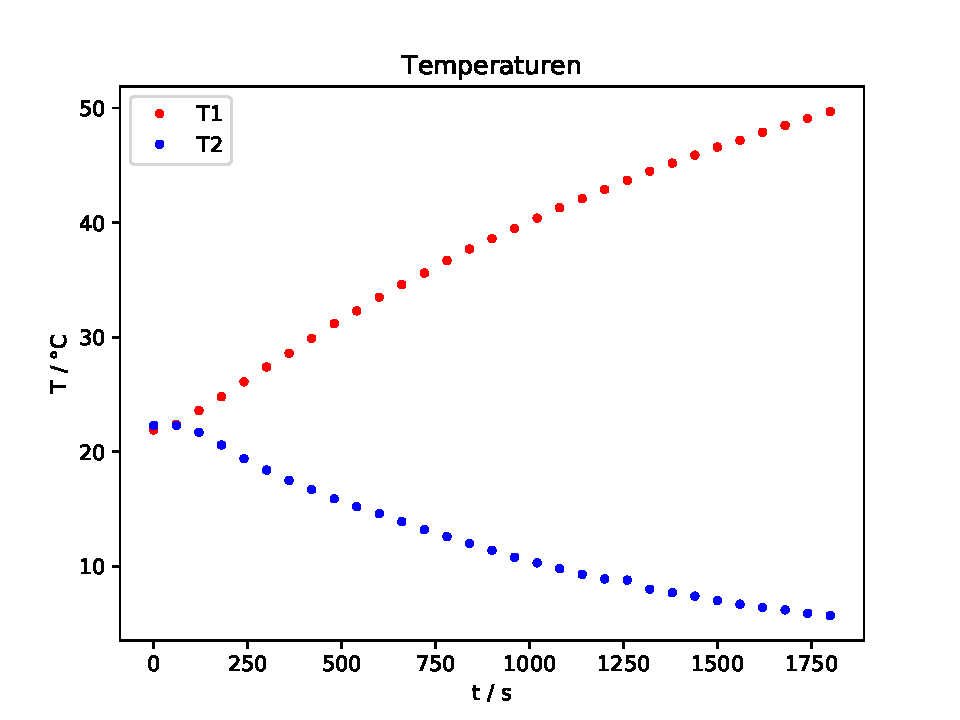
\includegraphics{build/Temperaturen.pdf}
  \caption{Die Temperaturen der Wärmereservoire.}
  \label{fig:Temperaturen}
\end{figure}

\subsection{Parameter der Regressionskurve}
Für die Regressionskurve wird die Funktion $T(t) = At^2 + Bt + C$ verwendet. Die
Parameter A, B, C und deren jeweilige Fehler für $T_2$ betragen:
\begin{align*}
  A &= (3.67 \pm 0.15) \cdot 10^{-6} \frac{\symup{K}}{\symup{s^2}} \\
  B &= (-1.61 \pm 0.03) \cdot 10^{-2} \frac{\symup{K}}{\symup{s}}  \\
  C &= (296.15 \pm 0.11) \cdot  \symup{K}
\end{align*}
Für $T_1$ ergeben sich folgende Parameter:
\begin{align*}
  A &= (-3.87 \pm 0.13) \cdot 10^{-6} \frac{\symup{K}}{\symup{s^2}} \\
  B &= (2.28 \pm 0.02)  \cdot 10^{-2} \frac{\symup{K}}{\symup{s}}  \\
  C &= (294.26 \pm 0.10 )\cdot \symup{K}
\end{align*}
\subsection{Bestimung von vier Differentialquotienten von $T_1$}
Die Differentialquotienten der Temperaturen $T_1$ und $T_2$ werden für vier verschieden
Zeiten berechnet. Die vier Messzeiten sind 600, 900, 1200 und 1500 Sekunden. Der
Differentialquotient ist
\begin{equation}
  \frac{\symup{d}T}{\symup{d}t} = 2At + B .
\end{equation}
Somit ergeben sich folgende Werte:
\begin{table}
  \centering
  \caption{Gemessene und berechnete Werte}
  \label{tab:Parameter}
  \begin{tabular}{c c c c c}
    \toprule
    $t/$s & $T_1/$K & $\frac{\symup{d}T_1}{\symup{d}t}/\left(10^{-2}\frac{\symup{K}}{\symup{s}}\right)$ & $T_2/$K & $\frac{\symup{d}T_2}{\symup{d}t}/\left(10^{-2}\frac{\symup{K}}{\symup{s}}\right)$  \\
    \midrule
      600 &  306.6 & $1.816 \pm 0.020$ & 287.8 & $-1.170  \pm 0.030$ \\
      900 &  311.8 & $1.583 \pm 0.020$ & 284.5 & $-0.949  \pm 0.030$ \\
      1200 & 316.0 & $1.351 \pm 0.020$ & 282.0 & $-0.729 \pm 0.030$ \\
      1500 & 319.8 & $1.119 \pm 0.020$ & 280.1 & $-0.509 \pm 0.030$ \\
   \bottomrule
 \end{tabular}
\end{table}

%Die Standardabweichungen werden hier mit dem Python-Package "Uncertainties" \cite{uncertainties} berechnet,
%welches die Gaußsche Fehlerfortpflanzung  \\
%\begin{equation}
%  \sigma_f = \sqrt{
%    \sum\limits_{i = 1}^N
%      \left( \frac{\partial f}{\partial x_i} \sigma_i \right)^{\!\! 2}
%    }
%\end{equation}
%nutzt.
\subsection{Berechnung der Güteziffern}
Die Güteziffer $\nu$ wird für die berechneten Differentialquotionenten mit zugehörigem Fehler mit Gleichung (9) bestimmt.
Dabei beträgt die Wärmekapazität des Wassers 4,18 $\frac{J}{gK}$ \cite{sample1}.
Die idealen Güteziffern werden mit der Formel
\begin{equation}
  \nu_{ideal} = \frac{T_1}{T_1-T_2}
\end{equation}
ermittelt. Es ergeben sich folgende Werte:
\begin{table}
  \centering
  \caption{Güteziffern}
  \label{tab:Reale und ideale Güteziffern}
  \begin{tabular}{c c c c}
    \toprule
    $t/$s & $\nu_{real}$ & $\nu_{ideal}$ & Abweichung \\
    \midrule
     600 & $2.538 \pm 0.028$ &   16.309 &  84.4\% \\
     900 & $2.212 \pm 0.028$ &   11.421 &  80.6\% \\
    1200 & $1.888 \pm 0.028$ &    9.294 &  79.6\% \\
    1500 & $1.564 \pm 0.028$ &    8.055 &  80.5\% \\
    \bottomrule
  \end{tabular}
\end{table}

Es wird eine deutliche Abweichung erkennbar. Die ideale Güteziffern setzen
voraus, dass der Prozess reversibel ist und, dass der Kompressor adiabatisch
komprimiert. Beides kann in der Realität nicht vollständig umgesetzt werden. Außerdem
geht über die Zeit Wärme verloren, was ebenfalls nicht den idealen Vorraussetzungen entspricht.
\subsection{Bestimmung des Massendurchsatzes}
Der Massendurchsatz lässt sich mit den Gleichungen (10) und (11) bestimmen. Zunächst
wird die Verdampfungswärme ermittelt. Dafür wird der natürliche Logarithmus von
$\frac{p_b}{p_0}$ als Funktion von $\frac{1}{T_1}$ aufgetragen. Die Steigung der sich ergebenden
Geraden ist die Verdampfungswärme $L$ \cite{sample2}.
\begin{figure}[H]
  \centering
  \includegraphics{build/Verdampfungswaerme.pdf}
  \caption{Ausgleichsgerade zur Bestimmung der Verdampfungswärme.}
  \label{fig:Verdampfungswaerme}
\end{figure}
Die Gerade kann durch die Gleichung
\begin{equation}
  y = (-1865 \pm 108)x + (8.22 \pm 0.35)
\end{equation}
beschrieben werden.
Die Verdampfungswärme beträgt dann $L = (-15513 \pm 903)$J.
Für $m_kc_k$ wird $750 \frac{\symup{J}}{\symup{K}}$ verwendet und $m_1c_w$ beträgt \SI{16720}{\joule\per\kelvin}.
Es ergeben sich folgende Massendurchsätze mit zugehöriger Abweichung:
\begin{table}[H]
  \centering
  \caption{Massendurchsätze}
  \label{tab:Massendurchsätze}
  \begin{tabular}{c c}
    \toprule
    $\frac{\Delta m}{\Delta t}/\frac{\symup{g}}{\symup{s}}$ & Fehler \\
    \midrule
    -1.70 & 0.10 \\
    -1.38 & 0.09 \\
    -1.05 & 0.08 \\
    -0.74 & 0.06 \\
    \bottomrule
  \end{tabular}
\end{table}
Um den Massendurchsatz in $\frac{\symup{g}}{\symup{s}}$ zu erhalten muss er noch
mit der Molaren Masse von Dichlordiflourmethan multipliziert werden.
Diese beträgt $120.9\frac{\symup{g}}{\symup{mol}}$.
\subsection{Bestimmung der mechanischen Kompressorleistung}
Die mechanische Kompressorleistung $N_{mech}$ lässt sich mit Gleichung (15) berechnen. Die dafür
benötigten Größen werden der Anleitung[1] entnommen und betragen:
\begin{align}
  \rho = \SI{5.51}{\kilo\gram\per\cubic\meter} \\
  \kappa = 1.14
\end{align}
Um die Dichte den vorhandenen Bedingungen anzupassen wird die ideale Gasgleichung
verwendet. Es gilt:
\begin{equation}
  \rho = \frac{\rho_0 T_0 p_a}{T_2 p_0}
\end{equation}
Für die Kompressorleistung und dessen Fehler folgt:
\begin{table}
  \centering
  \caption{Mechanische Kompressorleistung}
  \label{tab:Mechanische Kompressorleistung}
  \begin{tabular}{c c c c}
    \toprule
    t / s  &$\rho/\frac{\symup{g}}{\symup{m^3}}$ & $N_{mech}/$W & Fehler \\
    \midrule
     600 & 23094.1369 & -19.9 & 1.2 \\
     900 & 20994.6699 & -21.3 & 1.4 \\
    1200 & 19944.9364 & -19.7 & 1.4 \\
    1500 & 19420.0696 & -15.0 & 1.3 \\
    \bottomrule
  \end{tabular}
\end{table}
